\section{Capacity expansion - What is the problem?}

\subsection{Peak Load Pricing}

\subsubsection{optimal and perfectly competitive Peak load Pricing}

In electricity markets, demand varies from hour to hour and as it is not storable, it has to be met at any time of the day. If capacities are a binding constraint, there has to be rationing by rising prices. Of course, such rationing causes Welfare to decrease. On the other hand however, there are capacity costs. The literature on peak load pricing provides results on how to balance these two effects optimally. Under perfect competition, Prices will equal marginal costs in low demand periods $v=p$ (variable costs = price) and marginal costs plus a scarity rent in high demand periods. Under the assumption that there are fixed capacity costs $(c)$ how much capacity $(K)$ should be built taking into account that demand is not always high and there is a chance of $\pi$ to have high demand. The premium of the market price over marginal costs in peak periods multiplied with the chance of actually having a period of high demand reflects the value of increasing capacity by one unit $((p^p-v)\pi)$. (In off peak periods, the corresponding premium equals zero, reflecting the fact that in such states capacity is of no value.) This value of increasing capacity by one unit must equal capacity costs per unit $((p^p-v)*\pi)=(c)$ if this condition is met, social surplus is maximised and costs are minimised. A profit maximising firm under perfect competition would invest until exactly this condition is satisfied. So under perfect competition, one could rely on the market to provide optimal incentives for capacity investments (\cite{Fehr1994}).

\begin{figure}[h]
\centering
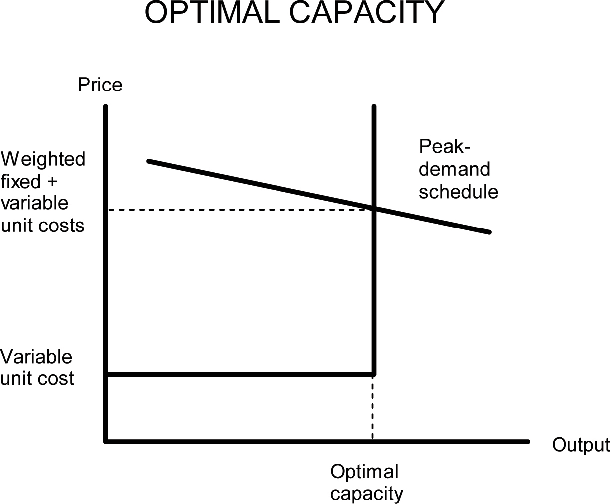
\includegraphics[width=.5\textwidth]{capacity/peak_load_opt}
      \label{peak_load_opt}
      \caption{Optimal Capacity}
      source: vor der Fehr and Harbord (1994)     
\end{figure}

Please note that we do not account for possible outages or rationing costs here although this is discussed in the literature. If capacity is too small in our case it can be seen in peak period prices which are higher than the long run incremental costs of capacity.

\subsubsection{Peak load pricing under Imperfect Competition}

If there is market power e.g. in the situation of an oligopoly this is not necessarily the case as prices which are distorted upwards may induce overinvestments. The situation of too high prices is depicted in figure \ref{peak_load_toohigh}. 

\begin{figure}[h]
\centering
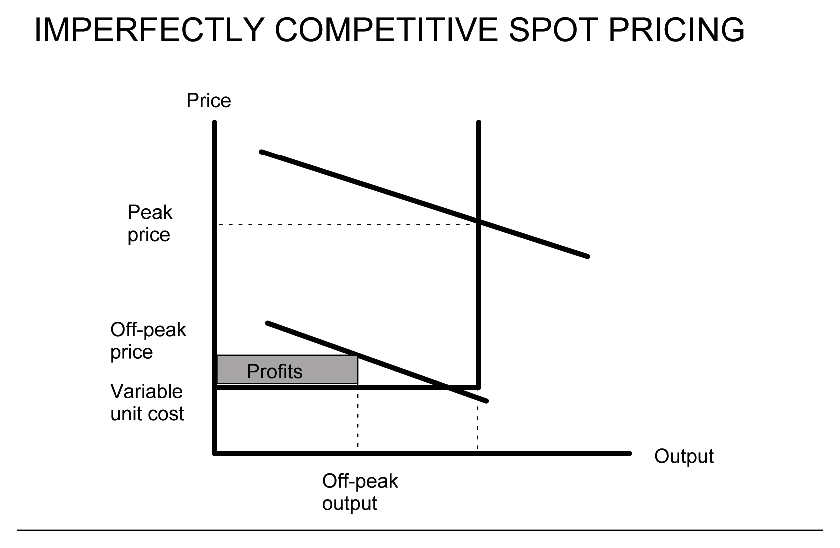
\includegraphics[width=.5\textwidth]{capacity/peak_load_toohigh}
      \label{peak_load_toohigh}            
      \caption{imperfectly competitive spot pricing}
       source: vor der Fehr and Harbord (1994)
\end{figure}

On the other side however, firms might have an incentive to cut on investments, thereby driving up the price in peak periods and increasing their profits. This, of course would only work if there are barriers to entry beyond the unit costs of investment which are $(c)$. This can be seen in figure \ref{peak_load_insufficient}.

\begin{figure}[h]
\centering
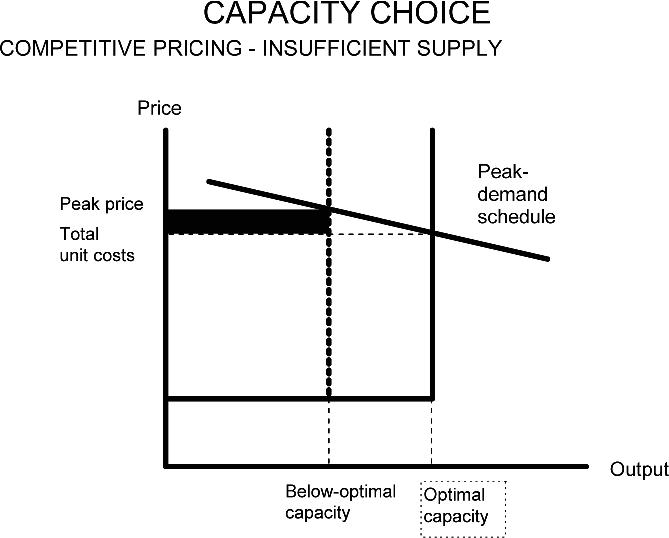
\includegraphics[width=.5\textwidth]{capacity/peak_load_insufficient}
      \label{peak_load_insufficient}            
      \caption{insufficient supply}
       source: vor der Fehr and Harbord (1994)
\end{figure}

While the socially optimal incentive to invest is still the same as above, a firm gets the following expected revenue per unit of investment:

\begin{equation}
	1/2 (1-\pi) (p^{op}-v) + \pi (w^p(K)+\frac{\partial w^p(K^*)}{\partial q}-v) - c
\end{equation}

The first part of the equation stands for possible gains of the investment that might occur during low peak periods. For simplicity we assume that there is a duopoly and a probability of $1/2$ for a new unit of capacity to be utilised. This is then multiplied by the probability to not have a peak period and the oligopoly price minus variable costs. In such periods it is possible to steal business, you would normally not have, from another firm. Such an effect can create an additional incentive to invest in capacity. As we shall see later on, this effect can be called a strategic effect of investments as well.

The second part of the equation stands for what the investing firm gains during peak periods. This equation is essentially the same as before, apart from the term ($w^{\acute{c}}$) which measures the reduction in the peak price which is due to the decreased scarity of capacity. This effect has to be taken into account now, as we switched from perfect competition to oligopoly.

So if the loss firms expect due to losses in the peak load market price are bigger than the gains due to more market share in off peak periods firms will underinvest as their incentive to invest is smaller than the optimal level under perfect competition. Of course, if the effect doe to business stealing is higher, firms will overinvest. So in an oligopolistic setting, firms will in general not choose an optimal level of investments and it cannot be said whether they will over- or underinvest (\cite{Fehr1994}). As we shall see later on, in a two stage game, strategic effects can be accounted for in different ways which has an effect on the predictions made.

\subsection{Optimal Technology Mix}

If demand were certain and constant, only one technology (the one which reaches the lowest possible costs in a standard cost minimization problem with capacity costs and operating costs as inputs) would be used \citep[see][pg. 183]{Chao1983}. This can be seen in the following graph (\ref{technology_choice_chow}) in which a standard cost minimization problem with capacity costs and operating costs as inputs and different technologies are shown. The minimal cost combination given input prices would be technology one. But when demand is uncertain or variable and the output is nonstorable some idle capacity becomes inevitable. This makes less capital intensive technologies such as 2 and 3 more attractive which would be dominated without fluctuations. However, all technologies which are not on the lower envelope are still inferior.

\begin{figure}[h]
\centering
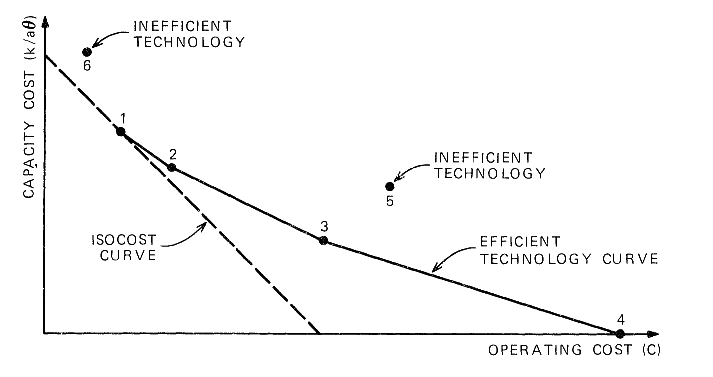
\includegraphics[width=.5\textwidth]{capacity/technology_choice_chow}
      \label{technology_choice_chow}            
      \caption{different technologies}
       source: Chow (1983)
\end{figure}

\cite{sherali1982} present a graphical illustration on how to find the optimal mix of different technologies if demand varies. Figure \ref{technology_choice_sherali} \textbf{b} shows the so - called load duration curve which plots the hours of the year ordered according to their energy demand. It can be seen, that only during a few hours of the year demand is very high. Figure \ref{technology_choice_sherali} \textbf{a} shows the cost curves of three different technologies. Technology three has low yearly fixed costs ($c_3$) and high variable costs ($f_3$) so if it would be used for more than $\alpha_{23}$ hours in a year it would be cheaper to use technology two instead. For most of the time of the year, it is actually cheaper to use technology one only which has fairly high fixed but low variable costs. The condition of when one technology becomes cheaper than the other is the same than the one derived by \cite{chow1983} (who also adds an additional stochastic element however). This condition for an optimal technology mix has first been advanced by \cite{Turvey1968}. Also \cite{Pineau2007} uses this condition.

\begin{eqnarray}
	c_1 + f_1 \alpha_{12} = c_2 + f_2 \alpha_{12}
	\alpha_{12} = \frac{c_2-c_1}{f_1-f_2}
\end{eqnarray}

This so called optimal running time can be translated into optimal investments into capacity of technology one two and three as can be seen in figure \ref{technology_choice_sherali} \textbf{b}.

\begin{figure}[h]
\centering
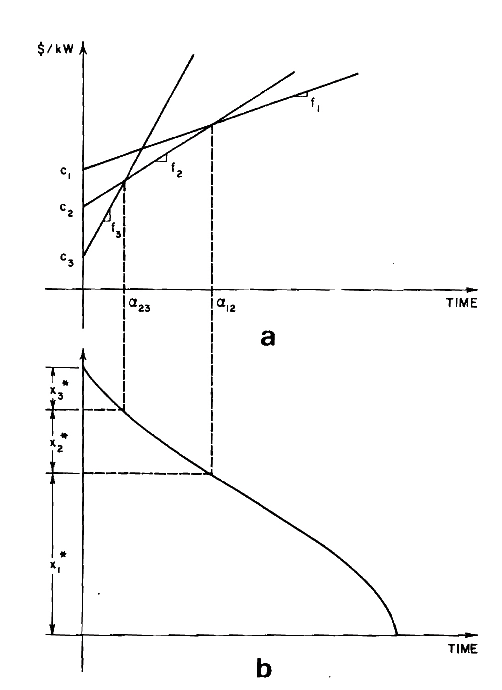
\includegraphics[width=.5\textwidth]{capacity/technology_choice_sherali}
      \label{technology_choice_sherali}            
      \caption{the load duration curve and cost curves - graphical determination of the optimal technology mix}
      source: Sherali et. al. (1982)
\end{figure}

What can be seen here is that which kind of capacity is optimal to be built depends on where demand actually increases. It is an unresolved issue whether competition and markets, be it perfect competition or imperfect forms alter the technology mix firms have an incentive to install in any way.

